\documentclass[conference]{IEEEtran}

\usepackage{cite}
\usepackage{amsmath}
\usepackage{amssymb}
\usepackage{url}
\usepackage{graphicx}
\usepackage{booktabs}
\usepackage{microtype}
\usepackage[table]{xcolor}
\usepackage{tikz}
\usetikzlibrary{positioning,arrows.meta}
\usepackage[hidelinks]{hyperref}

\definecolor{networkblue}{RGB}{52,152,219}
\definecolor{envgreen}{RGB}{46,204,113}
\definecolor{algorange}{RGB}{230,126,34}
\definecolor{allocpurple}{RGB}{155,89,182}

\title{Fair Contextual Bandits for Equitable
Diagnostic Decision-Making Under Missing Context}

\author{
\IEEEauthorblockN{Piter Z. Garcia Bautista}
\IEEEauthorblockA{MS Data Science / Bioinformatics\\Rochester Institute of Technology\\pizg8794@g.rit.edu}
\and
\IEEEauthorblockN{Daniel Krutz, Travis Desell}
\IEEEauthorblockA{Department of Software Engineering, Data Science\\Rochester Institute of Technology\\dxkvse@g.rit.edu, tjdvse@g.rit.edu}
}

\begin{document}
\maketitle


\section{Introduction}
This project develops a practical, reproducible framework for fairness-aware contextual
multi-armed bandits (CMAB/iCMAB) to make sequential decisions under uncertainty and limited
resources while treating algorithmic fairness as a first-class objective. The work focuses
on measuring and improving fairness across two domains---clinical diagnostic-like decision
workflows and quantum-network routing---by evaluating the same policy stack in a
simulation-first diagnostic environment and in a quantum-network routing simulator, with
time-evolving disparity reporting and at least one mitigation mechanism.
Two prior works provide the concrete testbeds used in this work: a clinical
diagnostic--motivated fairness audit and mitigation pipeline in equitable bioinformatics
\cite{garcia2025equitable_bioinformatics} and a threat-aware quantum-network routing study
using hybrid contextual bandits \cite{garcia2026threat_aware_quantum_routing}.
From a real-world perspective, the quantum routing testbed can be interpreted as online
resource allocation: deciding how to route competing flows when link success is uncertain and
network conditions change over time, while ensuring equitable service outcomes across groups.
Critically, the two-domain design also enables a cross-domain transfer study: after improving
performance and fairness within each domain, the framework tests whether policies developed in
one domain remain effective and equitable when applied to the other, focusing on transfer of
\emph{fairness mechanisms and policy-update strategies} rather than domain-specific features.

This survey reviews prior work needed to support this framework, including bandit foundations,
contextual/linear bandits and evaluation, learning under distribution shift and
missing/partial context (including group-dependent missingness/measurement noise), and
fairness definitions and fairness in bandit-style learning. It also includes domain grounding
for clinical disparities and quantum-network routing. The conclusion summarizes gaps and
clarifies how the proposed work differentiates itself by explicitly tracking and mitigating
disparities over time while testing transfer across both domains.


\section{Background}
Many real-world workflows in both clinical diagnostics and quantum-network routing require
sequential choices under uncertainty, resource constraints, and distribution shift. These
settings can amplify inequities when some groups systematically have lower-quality context
or different error profiles. This survey frames these workflows as a contextual bandit
problem: at each step, choose an action (an ``arm'') given observed context to maximize
utility while controlling fairness gaps.
In both domains, outcomes are stochastic and history-dependent: the reward distribution can
drift over time as conditions evolve, feedback is partial (bandit feedback), and context can
be delayed, noisy, or missing.

\subsection{Multi-armed bandits and contextual bandits}
In both domains, multi-armed bandits formalize online decision-making with
exploration--exploitation tradeoffs: at each round $t$ an agent chooses an action
$a_t \in \{1,\ldots,K\}$ and observes reward $r_t$ only for the chosen arm (bandit feedback).
Performance is measured by \emph{cumulative regret}:
\begin{equation}
R_T = \sum_{t=1}^{T} \bigl(\mu^* - \mu_{a_t}\bigr)
\label{eq:regret}
\end{equation}
where $\mu^* = \max_k \mu_k$ is the optimal arm mean and $\mu_{a_t}$ is the mean reward of
the chosen arm. A policy is desirable if $R_T = o(T)$, meaning the per-step loss vanishes
over time.

Contextual bandits extend this setting by conditioning action choice on a context vector
$\mathbf{x}_t \in \mathbb{R}^d$ observed before each decision. The LinUCB
algorithm~\cite{li2010contextual} maintains a ridge regression estimate
$\hat{\boldsymbol{\theta}}_a$ per arm and selects actions via:
\begin{equation}
a_t = \arg\max_{a} \Bigl(
  \mathbf{x}_t^\top \hat{\boldsymbol{\theta}}_a
  + \alpha \sqrt{\mathbf{x}_t^\top \mathbf{A}_a^{-1} \mathbf{x}_t}
\Bigr)
\label{eq:linucb}
\end{equation}
where $\mathbf{A}_a$ accumulates outer products of context vectors and $\alpha$ controls
exploration. Contextual policies can improve sample-efficiency and stability when the context
is predictive of outcomes; however, when context is missing or systematically noisier for
some groups, these policies can inadvertently encode and amplify measurement inequities.

\subsection{Fairness in sequential decision-making}
Fairness in supervised learning is commonly operationalized through group-based error
disparities. Let $Y \in \{0,1\}$ be a binary outcome, $\hat{Y}$ a predicted label, and
$A \in \{0,1\}$ a protected group attribute. \emph{Equality of opportunity}~\cite{hardt2016equality}
requires equal true positive rates across groups:
\begin{equation}
P(\hat{Y}=1 \mid Y=1, A=0) \;=\; P(\hat{Y}=1 \mid Y=1, A=1)
\label{eq:eqopp}
\end{equation}
\emph{Equalized odds} additionally requires equal false positive rates. In a bandit setting,
fairness must be tracked over time under partial feedback and changing conditions, making it
important to monitor time-evolving disparities (e.g., FNR/FPR gaps, not only aggregate averages)
and to apply
mitigation during the policy update loop rather than only post-hoc.

\subsection{Domain grounding: diagnostics and quantum routing}
In the quantum-network routing domain, routing decisions act as online resource allocation
under probabilistic link success, limited entanglement/quantum-resource availability, and
time-varying congestion;
context may include link-quality estimates and network load/queue signals, but these signals
can be delayed, noisy, or partially observed. In this project, service equity is defined as parity in
routing outcomes (e.g., success probability/latency parity across flow groups) under these
constraints. Both domains share a common mathematical structure: stochastic, history-dependent
dynamics with non-stationarity, partial context, and compounding decisions over time.
In clinical diagnostics, context may include patient features, test and
sample-quality indicators, and operational constraints, but access to context can be
incomplete or systematically noisier for some populations. These limitations create
performance and fairness risks, especially when optimizing aggregate performance, which can
hide subgroup error spikes (e.g., false-negative gaps) unless the system is explicitly
monitored and constrained. Unlike many evaluations that report utility-only bandit performance
or post-hoc fairness for static predictors, the proposed work makes the time-evolving
utility--fairness tradeoff explicit and tests transfer across both domains.
These testbeds are described in Section~\ref{sec:related_testbeds}.


\section{Related Work}
Table~\ref{tab:overview} gives a compact map of the works reviewed and how they support
the proposed project.

\begin{table*}[t]
\caption{High-level overview of related works reviewed in this survey.}
\centering
\small
\begin{tabular}{p{0.28\textwidth} p{0.68\textwidth}}
\toprule
Category & Representative works \\
\midrule
Primary project testbeds (two prior works)
  & Equitable bioinformatics (clinical diagnostic motivation) \cite{garcia2025equitable_bioinformatics};
    threat-aware quantum routing bandit evaluation \cite{garcia2026threat_aware_quantum_routing} \\
Bandit foundations (exploration--exploitation basics)
  & UCB analysis \cite{auer2002finite};
    Thompson sampling tutorial \cite{russo2018tutorial};
    bandit textbook \cite{lattimore2020bandit} \\
Contextual/linear bandits (side information + evaluation)
  & Epoch-Greedy \cite{langford2007epoch};
    contextual bandits in practice \cite{li2010contextual};
    linear bandits \cite{abbasi2011linear};
    scalable CB \cite{agarwal2014taming};
    offline evaluation \cite{dudik2011doubly} \\
Shift / partial context (missingness + nonstationarity)
  & Non-stationary UCB \cite{garivier2008ucb};
    non-stationary rewards \cite{besbes2014stochastic};
    restricted context \cite{bouneffouf2017context};
    unobserved contexts \cite{park2022efficient} \\
Fairness (definitions + constraints in sequential learning)
  & Equality of opportunity \cite{hardt2016equality};
    fairness in bandits \cite{joseph2016fairness};
    fairness in RL \cite{jabbari2017fairness};
    offline fairness guarantees \cite{metevier2019offline};
    fair contextual MABs \cite{chen2020fair};
    clinical bias case study \cite{obermeyer2019dissecting} \\
Quantum networking (routing under uncertainty + resource scarcity)
  & Quantum internet vision \cite{wehner2018quantum};
    entanglement routing \cite{pant2019routing};
    optimal quantum routing \cite{caleffi2017optimal} \\
\bottomrule
\end{tabular}
\label{tab:overview}
\end{table*}

\subsection{Primary project testbeds (two prior works)}
\label{sec:related_testbeds}

\subsubsection{Equitable bioinformatics for diagnostic-relevant fairness auditing}
Garcia Bautista~\cite{garcia2025equitable_bioinformatics} presents a fairness-audit and
mitigation framework (EQUITAS) for diagnostic-relevant bioinformatics pipelines, using RNA
secondary-structure prediction as a case study. The work fine-tunes an Enhanced Nussinov
dynamic-programming model with Optuna-driven hyperparameter search and evaluates it alongside
five baselines on a curated dataset of 20 RNA sequences spanning multiple RNA types and
compositional bins, reporting both performance and fairness metrics across protected attributes
such as sequence type, GC-content bins, and length bins. Post-processing calibration and
fairness-aware dataset augmentation are used to correct disparate-impact violations, achieving
80\% rule compliance across algorithms. A limitation for the proposed project is that this
study is largely an offline, static evaluation rather than an online sequential decision problem
with bandit feedback; it motivates clinical-domain fairness metrics and context-quality concerns
but does not model exploration--exploitation or time-evolving disparities.

\subsubsection{Threat-aware quantum routing via hybrid contextual bandits}
Garcia Bautista~\cite{garcia2026threat_aware_quantum_routing} evaluates contextual, adversarial,
and hybrid bandit algorithms for joint quantum entanglement routing and resource allocation
under non-stationary and adversarial conditions. The study compares 13 algorithms across
multiple threat scenarios and reports that pursuit--neural hybrid variants provide robust
performance under strategic attacks; it further validates robustness trends via cross-testbed
evaluation across external quantum-network simulators. This work grounds the quantum-network
routing testbed used in the proposed project by providing domain-realistic uncertainty, resource
constraints, and adversarial shifts. A limitation for the proposed project is that robustness is
the primary focus; explicit outcome-based fairness/service-equity monitoring is not central and
will be added in the shared evaluation framework.

\begin{figure}[t]
\tiny
\centering
\resizebox{0.9\columnwidth}{!}{%
    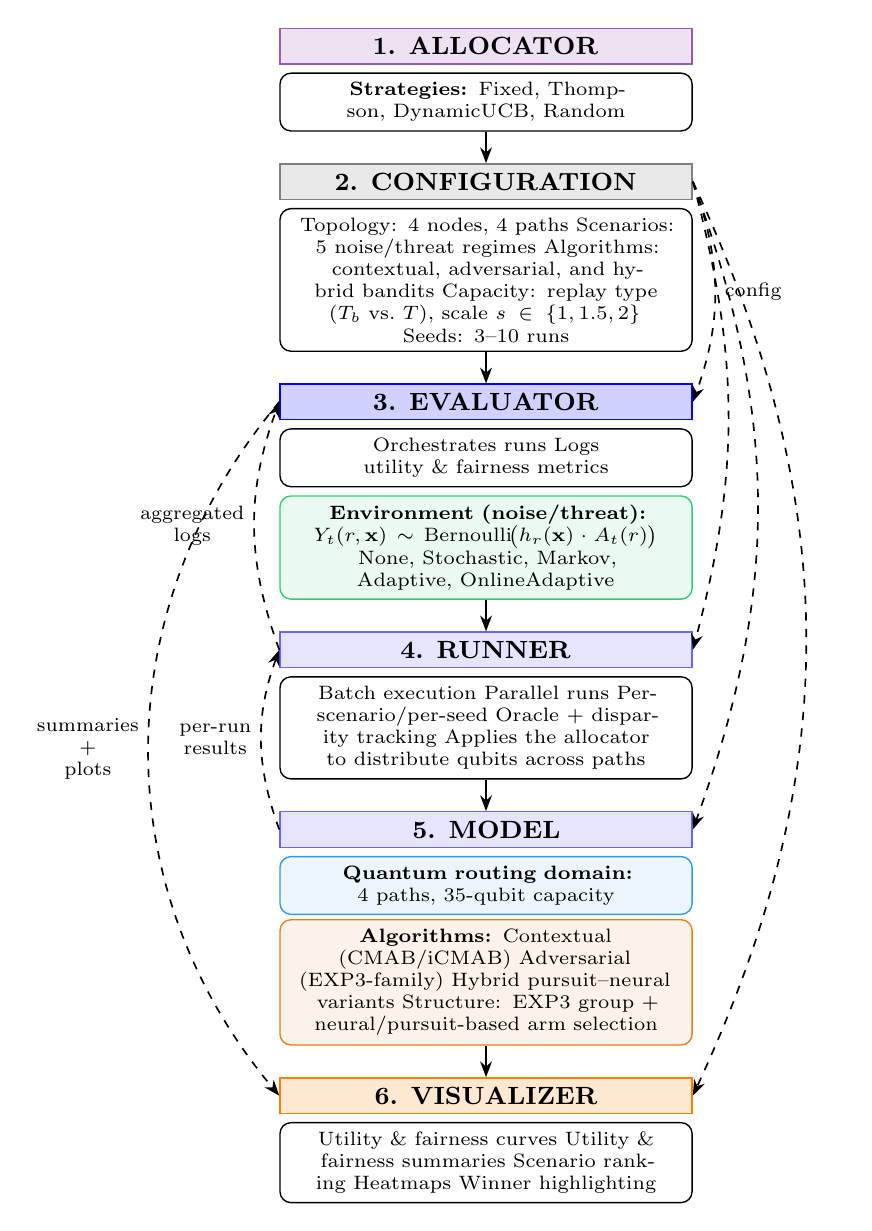
\begin{tikzpicture}[
      node distance=0.5cm,
      block/.style={rectangle, draw, fill=white, text width=5.0cm, text centered, rounded corners, minimum height=0.1cm, line width=0.5pt},
      layer/.style={rectangle, draw, fill=white, text width=5.0cm, text centered, minimum height=0.1cm, line width=0.5pt, font=\small},
      arrow/.style={-Stealth, line width=0.6pt},
      lab/.style={font=\scriptsize}
    ]

    \node[layer, fill=allocpurple!18, draw=allocpurple] (alloc) {\textbf{1. ALLOCATOR}};
    \node[block, below=0.1cm of alloc, font=\scriptsize] (alloccontent) {
      \textbf{Strategies:} Fixed, Thompson, DynamicUCB, Random
    };

    \node[layer, fill=gray!18, draw=gray, below=0.4cm of alloccontent] (config) {\textbf{2. CONFIGURATION}};
		    \node[block, below=0.1cm of config, font=\scriptsize] (configcontent) {
		      Topology: 4 nodes, 4 paths
		      Scenarios: 5 noise/threat regimes
		      Algorithms: contextual, adversarial, and hybrid bandits
		      Capacity: replay type ($T_b$ vs.\ $T$), scale $s\in\{1,1.5,2\}$\\
		      Seeds: 3--10 runs
		    };

	    \node[layer, fill=blue!18, draw=blue, below=0.4cm of configcontent] (evaluator) {\textbf{3. EVALUATOR}};
	    \node[block, below=0.1cm of evaluator, font=\scriptsize] (evalcontent) {
	      Orchestrates runs
	      Logs utility \& fairness metrics
	    };
	    \node[block, below=0.1cm of evalcontent, font=\scriptsize, fill=envgreen!10, draw=envgreen] (env) {
	      \textbf{Environment (noise/threat):}
	      $Y_t(r,\mathbf{x}) \sim \mathrm{Bernoulli}\!\big(h_r(\mathbf{x}) \cdot A_t(r)\big)$
	      None, Stochastic, Markov, Adaptive, OnlineAdaptive
	    };

	    \node[layer, fill=blue!10, draw=blue!60, below=0.4cm of env] (runner) {\textbf{4. RUNNER}};
	    \node[block, below=0.1cm of runner, font=\scriptsize] (runnercontent) {
	      Batch execution
	      Parallel runs
	      Per-scenario/per-seed Oracle + disparity tracking
	      Applies the allocator to distribute qubits across paths
	    };

	    \node[layer, fill=blue!10, draw=blue!60, below=0.4cm of runnercontent] (model) {\textbf{5. MODEL}};
	    \node[block, below=0.1cm of model, font=\scriptsize, fill=networkblue!10, draw=networkblue] (net) {
	      \textbf{Quantum routing domain:}
	      4 paths, 35-qubit capacity
	    };
		    \node[block, below=0.05cm of net, font=\scriptsize, fill=algorange!10, draw=algorange] (algo) {
		      \textbf{Algorithms:}
		      Contextual (CMAB/iCMAB)
		      Adversarial (EXP3-family)
		      Hybrid pursuit--neural variants
		      Structure: EXP3 group + neural/pursuit-based arm selection
		    };

	    \node[layer, fill=orange!18, draw=orange, below=0.4cm of algo] (visualizer) {\textbf{6. VISUALIZER}};
	    \node[block, below=0.1cm of visualizer, font=\scriptsize] (viscontent) {
	      Utility \& fairness curves
	      Utility \& fairness summaries
	      Scenario ranking
	      Heatmaps
	      Winner highlighting
	    };

    \draw[arrow] (alloccontent.south) -- (config.north);
    \draw[arrow] (configcontent.south) -- (evaluator.north);
    \draw[arrow] (env.south) -- (runner.north);
    \draw[arrow] (runnercontent.south) -- (model.north);
    \draw[arrow] (algo.south) -- (visualizer.north);

    \draw[arrow, dashed, bend left=20] (config.east) to node[lab, right] {config} (evaluator.east);
    \draw[arrow, dashed, bend left=15] (config.east) to (runner.east);
    \draw[arrow, dashed, bend left=20] (config.east) to (model.east);
    \draw[arrow, dashed, bend left=25] (config.east) to (visualizer.east);

    \draw[arrow, dashed, bend left=20] (model.west) to node[left, lab, align=center] {per-run\\results} (runner.west);
    \draw[arrow, dashed, bend left=20] (runner.west) to node[left, lab, align=center] {aggregated\\logs} (evaluator.west);
    \draw[arrow, dashed, bend right=40] (evaluator.west) to node[left, lab, align=center] {summaries\\+\\plots} (visualizer.west);
    \end{tikzpicture}
}
\vspace{-0.45cm}
\caption{\tiny Modular framework for quantum routing evaluation, following the evaluation
stack described in \cite{garcia2026threat_aware_quantum_routing}. The evaluation stack separates allocator,
configuration, evaluator, runner, model, and visualizer concerns to support systematic
ablation under consistent capacity and threat semantics.}
\label{fig:quantum_framework}
\end{figure}

\paragraph{Algorithmic framework (modular evaluation stack).}
The quantum-routing testbed in \cite{garcia2026threat_aware_quantum_routing} uses the layered
evaluation architecture shown in Figure~\ref{fig:quantum_framework}. At a high level, an
\emph{allocator} specifies a resource-distribution rule, a shared \emph{configuration} fixes
topology/scenarios/capacity semantics, an \emph{evaluator} orchestrates runs and logging, a
\emph{runner} executes batched scenarios under fixed seeds, a \emph{model} implements the
routing policy (bandit learner + network), and a \emph{visualizer} aggregates results into
plots and winner summaries. This modular structure is reused in the proposed work to add
fairness/service-equity monitoring and mitigation under the same experimental controls.
Having grounded the two experimental testbeds, the remainder of this section surveys the
algorithmic and fairness literature needed to design and evaluate a shared fairness-aware CMAB
framework across both domains.


\subsection{Bandit foundations and core algorithms}

\subsubsection{Upper confidence bound (UCB) analysis}
Auer et al.~\cite{auer2002finite} provide a foundational finite-time regret analysis for
multi-armed bandits and introduce UCB-style algorithms that choose actions using optimistic
confidence bounds, achieving gap-dependent regret logarithmic in $T$ under stochastic
assumptions (see Eq.~\ref{eq:regret}). A limitation for the proposed work is that standard
UCB assumes stationarity and does not incorporate context or group-based fairness constraints;
extensions are required for distribution shift, heterogeneous contexts, and explicit disparity
monitoring over time.

\subsubsection{Thompson sampling}
Russo et al.~\cite{russo2018tutorial} survey Thompson sampling as a Bayesian approach to
exploration--exploitation, highlighting strong empirical performance and the conceptual
simplicity of sampling from a posterior over rewards. Thompson sampling is attractive for the
proposed project as a baseline in both domains because it adapts to uncertainty naturally and
often performs well under limited feedback. However, typical implementations focus on
utility/regret and do not provide fairness guarantees; when context is missing or
systematically noisy for some groups, posterior updates can encode these measurement
inequities unless the model explicitly accounts for them.

\subsubsection{Bandit textbook perspective}
Lattimore and Szepesv\'{a}ri~\cite{lattimore2020bandit} provide a comprehensive reference on
bandit algorithms (stochastic, adversarial, contextual, linear), including proof techniques
and practical design choices. This text grounds algorithm selection and ablation design for
the proposed project. A practical limitation is that textbook settings generally assume
correctly observed context and utility-centric objectives; fairness-aware objectives and
missingness mechanisms must be layered on top.


\subsection{Contextual and linear bandits in practice}

\subsubsection{Epoch-Greedy contextual bandits}
Langford and Zhang~\cite{langford2007epoch} introduce the Epoch-Greedy algorithm, one of the
first contextual bandit algorithms with provable regret bounds. Their approach interleaves
exploration epochs (uniform arm selection for reward estimation) with exploitation epochs
(applying the current best policy), and shows that any supervised learning oracle can serve
as the reward estimator. This motivates the use of offline regression oracles within online
bandit policies---a strategy relevant to the iCMAB-style informed policy in the proposed
project. A limitation is the dependence on epoch length, which is often unknown in practice.

\subsubsection{Contextual bandits for personalization}
Li et al.~\cite{li2010contextual} demonstrate contextual bandits for news recommendation
using LinUCB (Eq.~\ref{eq:linucb}), showing how context enables personalized decisions while
balancing exploration and exploitation in a real deployment. The key limitation in the
proposed setting is that context can be incomplete and systematically lower-quality for some
populations, leading to performance disparities if policies are optimized only for average
reward.

\subsubsection{Linear stochastic bandits}
Abbasi-Yadkori et al.~\cite{abbasi2011linear} analyze linear stochastic bandits and provide
improved confidence ellipsoids for the unknown parameter vector $\boldsymbol{\theta}$,
achieving regret bounds that scale as $\tilde{O}(d\sqrt{T})$ under standard stochastic
assumptions. Linear contextual bandits are a key baseline for the proposed work because they
are simple, interpretable, and offer a clean place to inject missingness-handling and
fairness-aware penalties. A limitation is the linear modeling assumption: if the relationship
between context and outcome differs across groups or shifts over time, the model can underfit
and hide subgroup-specific error spikes.

\subsubsection{Scalable contextual bandits}
Agarwal et al.~\cite{agarwal2014taming} propose a computationally efficient reduction-based
approach to contextual bandits that makes it practical to use rich policy classes. This is
relevant to the proposed project as a template for scaling beyond simple linear models while
keeping training tractable. However, the work primarily optimizes reward and assumes
representative context; fairness auditing under group-dependent context quality requires
additional monitoring and constraints.

\subsubsection{Offline evaluation with bandit feedback}
Dud\'{i}k et al.~\cite{dudik2011doubly} develop doubly robust estimators for policy
evaluation and learning from bandit feedback, combining direct reward modeling with
inverse-propensity weighting. This is useful for the proposed project because it supports
evaluation and comparison of policies under partial feedback. A limitation is that estimator
validity depends on correct propensities and sufficient support in logged data; if groups
have different action distributions or context missingness rates, variance and bias can differ
by group, complicating fairness assessment.


\subsection{Distribution shift and missing/partial context}

\subsubsection{Non-stationary bandits: UCB with change detection}
Garivier and Moulines~\cite{garivier2008ucb} study UCB-style policies for non-stationary
bandit problems, motivating mechanisms such as discounting or sliding windows to adapt to
reward changes. This is relevant to both domains: patient mix and operational processes can
change, and network load and link conditions can vary over time. The limitation for the
proposed work is that non-stationary regret does not directly capture fairness; even if a
policy adapts quickly in aggregate, it may exhibit persistent group disparities if context
quality differs systematically across groups.

\subsubsection{Non-stationary rewards and variation budgets}
Besbes et al.~\cite{besbes2014stochastic} establish minimax-optimal rates for regret in
non-stationary bandit problems where arm means change subject to a total variation budget,
and propose a sliding-window UCB variant. A key finding is that ignoring non-stationarity
can lead to linear regret. The proposed project incorporates distribution shift as a
first-class experimental variable, testing bandit policies under both gradual and abrupt
shifts across both testbeds.

\subsubsection{Restricted context in contextual bandits}
Bouneffouf et al.~\cite{bouneffouf2017context} consider contextual bandits when only a
subset of context features can be observed at decision time, directly aligned with the
proposed project's focus on missing or unevenly measured context. The limitation is that
restricted-context selection is typically optimized for reward; extending the selection
mechanism to also reduce group disparities is not standard and is a key innovation
opportunity.

\subsubsection{Bandits with unobserved contexts}
Park and Faradonbeh~\cite{park2022efficient} address bandit control when contexts are
unobserved, proposing algorithms that learn to act effectively despite latent context.
This motivates algorithm designs that remain robust when the observed context is incomplete
or unreliable. A limitation is that fairness considerations are not central: if latent-context
recovery quality differs across groups due to unequal measurement, fairness risks persist
without explicit disparity tracking and mitigation.


\subsection{Fairness: definitions and fairness in bandit learning}

\subsubsection{Equality of opportunity and error-based fairness}
Hardt et al.~\cite{hardt2016equality} formalize equality of opportunity and related
group-based fairness criteria (Eq.~\ref{eq:eqopp}) in supervised learning, emphasizing that
fairness can be defined in terms of error rates conditioned on true labels (e.g., equalizing
false negative rates across groups). These definitions provide a clear measurement target for
the clinical domain, where false-negative disparities have high stakes. A limitation for the
proposed project is that supervised-learning fairness is typically evaluated post-hoc on
static predictors; sequential decision-making adds partial feedback and time dynamics, so
disparities should be measured as a function of time and policy behavior.

\subsubsection{Fairness in classic and contextual bandits}
Joseph et al.~\cite{joseph2016fairness} study fairness constraints in bandit learning and
analyze how fairness requirements change achievable regret. This work is central to the
proposed project because it directly links bandit exploration policies to fairness constraints
and highlights that naive utility optimization can be incompatible with fairness goals.
A limitation is that many fairness formulations in bandits rely on simplified assumptions;
the proposed project must operationalize group definitions and disparity metrics differently
for diagnostics (error gaps) and quantum routing (service equity).

\subsubsection{Fairness in reinforcement learning}
Jabbari et al.~\cite{jabbari2017fairness} study fairness in reinforcement learning, requiring
that a policy never takes an action that is unfair to any individual in expectation, and
provide algorithms with polynomial sample complexity. The key challenge they identify is that
fairness constraints can slow learning when group-specific feedback is sparse---directly
relevant to the clinical diagnostics domain, where some patient groups may have systematically
fewer observations, making it harder to estimate group-wise error rates accurately.

\subsubsection{Offline contextual bandits with high-probability fairness}
Metevier et al.~\cite{metevier2019offline} propose a method for offline contextual bandits
that provides high-probability guarantees that a deployed policy satisfies user-specified
fairness constraints, using importance-weighted estimators and Seldonian optimization.
A significant limitation is the offline setting assumption: the algorithm requires a fixed
logged dataset and does not address online fairness under distribution shift. The proposed
project extends this direction to the online setting, where fairness constraints must be
maintained continuously as the policy learns from streaming data.

\subsubsection{Fair contextual multi-armed bandits}
Chen et al.~\cite{chen2020fair} develop algorithms for fair contextual MABs that satisfy
group fairness constraints (parity in arm-selection rates across groups) while maintaining
sublinear regret, and characterize the utility--fairness tradeoff as a function of group
distribution imbalance. This is the most directly related prior work to the proposed project.
A key limitation is that their fairness criterion focuses on arm-selection parity rather than
outcome parity (e.g., FNR/FPR gaps), which may not capture the clinically or operationally
relevant disparities. The proposed project uses outcome-based fairness metrics that are more
directly interpretable in clinical and service-equity contexts, and extends the evaluation to
distribution shift and cross-domain transfer.

\subsubsection{Clinical bias case study motivating fairness audits}
Obermeyer et al.~\cite{obermeyer2019dissecting} analyze a widely used health-risk prediction
system and show how proxy targets can encode racial bias, producing systematic under-allocation
of care for Black patients at the same predicted risk. This motivates the proposed project's
emphasis on fairness auditing and on monitoring subgroup-specific errors rather than relying
on aggregate metrics. A limitation is that this work addresses static prediction/triage rather
than sequential decision policies; however, the mechanism is relevant: optimizing a proxy
objective under biased measurements can yield persistent disparities unless explicitly
corrected.


\subsection{Quantum networking and routing as a second testbed}

\subsubsection{Quantum internet: vision and engineering constraints}
Wehner et al.~\cite{wehner2018quantum} describe the vision for a quantum internet and outline
key engineering challenges, including entanglement generation, storage, and networking
protocols. This work provides domain background and motivates why routing decisions in quantum
networks face uncertainty and resource scarcity. A limitation is that fairness is not a
primary focus; the proposed project extends this domain by explicitly considering service
equity across user/flow groups when learning routing policies under uncertainty.

\subsubsection{Routing entanglement in the quantum internet}
Pant et al.~\cite{pant2019routing} develop methods for routing entanglement in quantum
networks, addressing how to select paths and manage entanglement distribution under
probabilistic link success. This motivates a concrete quantum routing decision process
suitable as a second testbed. The limitation for the proposed project is that routing work
is typically evaluated on throughput/fidelity metrics without group-based disparity
monitoring; the proposed work adds explicit service-equity tracking using a shared
fairness-aware contextual MAB evaluation stack.

\subsubsection{Optimal routing for quantum networks}
Caleffi~\cite{caleffi2017optimal} formulates quantum path selection as an optimization over
link fidelity, decoherence time, and entanglement generation rate, showing that shortest-path
routing significantly underperforms optimal routing due to the stochastic nature of link
success. A limitation is the assumption of a static network with known link statistics; in
practice, link quality varies dynamically. The proposed project extends the routing problem
to an online learning setting using contextual bandits, where link-quality context is observed
but statistics are unknown and shift over time.


\section{Conclusion}
Prior work provides strong foundations for multi-armed bandits, contextual/linear bandits,
and evaluation under bandit feedback, as well as clear fairness definitions and initial work
on fairness constraints in bandit learning. However, a gap remains at the intersection of:
(i) missing or unevenly measured context, (ii) time-varying conditions, and (iii) explicit,
time-evolving disparity monitoring and mitigation in sequential decision systems.

The proposed project differentiates itself by building a reusable framework that evaluates
fairness-aware contextual MAB policies under controllable missing-context mechanisms and
distribution shift, tracks group disparities over time, and tests transfer across two distinct
domains: clinical diagnostic-like decision-making and quantum-network routing. While
Chen et al.~\cite{chen2020fair} address fair contextual MABs and Joseph et al.~\cite{joseph2016fairness}
address fairness in bandit learning, to our knowledge existing work does not jointly evaluate
outcome-based disparity metrics (FNR/FPR gaps) under distribution shift and test transfer
across fundamentally different domains. This two-domain evaluation demonstrates that the
methodology is generic---not tuned to a single application---while remaining grounded in
domain-realistic constraints.
In particular, \cite{garcia2025equitable_bioinformatics,garcia2026threat_aware_quantum_routing}
serve as the two primary experimental foundations for the project’s cross-domain transfer study.
This transfer framing is relevant to high-uncertainty operational regimes (e.g., surges), where
decision policies must adapt under non-stationarity and partial observability rather than assuming
stable, i.i.d. data.

\noindent\textbf{Overleaf (editable):}
\url{https://www.overleaf.com/3621132125pfjhvkxzsbkp#0cab76}

\bibliographystyle{IEEEtran}
\bibliography{survey-references}

\end{document}
